\documentclass[10pt,conference,compsocconf]{IEEEtran}

%\usepackage{times}
%\usepackage{balance}
\usepackage{url}
\usepackage{graphicx}	% For figure environment
\usepackage{subcaption}


\begin{document}
\title{CIL: Road Segmentation}

\author{
  Igor Pesic\\
  Department of Computer Science,\\ ETH Zurich
  \and
  Felipe Sulser\\
  Department of Computer Science,\\ ETH Zurich
  \and
  Minesh Patel\\
  Department of Computer Science,\\ ETH Zurich
}

\maketitle

\begin{abstract}
  Image segmentation of the aerial road images has become a significant part of the research in the recent years.
  The use cases are numerous and we are going to focus on the simpler, but still very useful part, namely just the road
  segmentation. Our task is to classify the pixels as either road or background. To achieve our goal we have combined
  techniques proposed in several other papers and have adjusted these to suite our requirements and resources best as possible.  
  The main part of our solution is convolution neural network. Beside it we apply the techniques for data augmentation,
  feature selection and post-processing. The results we obtained with our solution are very close to the state-of-the-art
  solutions proposed in the other papers, but very often, our model is much simpler.
\end{abstract}

\section{Introduction}

The goal of this work is to segment out the road on the aerial images. The problem is to decide what pixels
represent the road and what pixels are not the road. Even though we would ideally like to have a pixel-wise
granularity, we are proposing the approach which achieves the patch-wise granularity which is many cases good enough,
especially in this project. This also simplifies the problem substantially since each patch has only value 0 or 1. \\
\\
We have implemented the solution which is combination of multiple similar other works on this topic (TODO: ref papers) 
and we have managed to achieve very similar results. The focus of our work was the design of the
convolutional-neural-network (CNN) but we also invested a substantial amount of effort into denoising in order
to improve the results obtained by CNN. We would also like to mention that because of constrained resources
we had to simplify some parts of our model.\\
\\
This report has the following structure: in Section \ref{sec:Data} we explain all the steps we do before training
and evaluating the model, in Section \ref{sec:model_and_methods} we describe our model, both CNN and denoising
that comes after that. Finally in \ref{sec:results} we discuss the results achieved with our model.


\section{Data}
\label{sec:Data}

\subsection{Data Augmentation}
\label{sec:data_aug}
The original data set consisted of 100 labeled aerial images of road maps. As our approach consists of a
deep neural network, we considered the given data not enough and thus we tried to augment it as much as possible.
First thing we did, was to rotate all the images by 90 degrees and to mirror them. Beside the obvious increase
in the training data size, this approach also makes our model more robust. Furthermore we have noticed that the 
predictions on the diagonal roads were much worse than on the horizontal and vertical ones. This was obviously due to
the lack of diagonal roads in our original data set. In order to fix this, we have picked 9 images with diagonal
roads and highways which we rotated again by 180 and 270 degrees. Finally, we have noticed some inconsistencies
in labeling of couple of images and we have decided to discard those from our training data. At the end our data set
had 309 images in total.

\subsection{Feature extraction}
\label{sec:feature}
In the baseline model we have split the image in patches of size $16\times16$ pixels. This provided granularity
that was good enough, but it lacked the information about the surroundings. In order to address that we have come up
with solution that we called \textit{added context}. Later, we have found the same approach in \cite{mthesis},
\cite{Mnih2010} and \cite{eth_paper}. The approach is as following: split the image in $16\times16$ patches, then add the 
surroundings area to it so that patches have the total size of $64\times64$ pixels. The difference between patches is
shown in \ref{fig:patches}. Labels are based solely on the original $16\times16$ patch. 

\begin{figure}
\centering
\begin{subfigure}{.5\columnwidth}
  \centering
  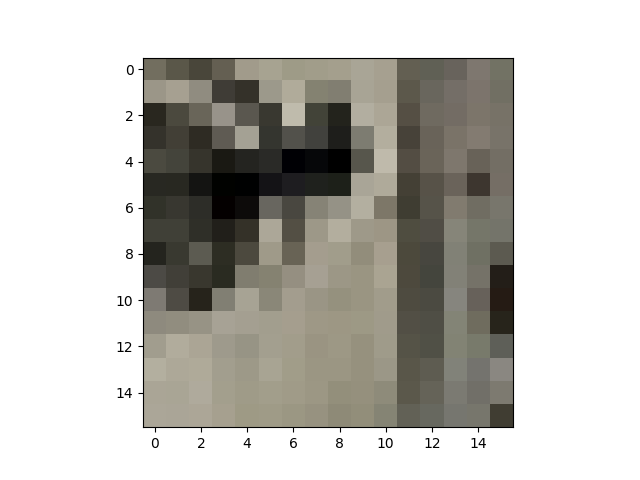
\includegraphics[width=.8\linewidth]{orig_patch.png}
  \caption{Original patch}
\end{subfigure}%
\begin{subfigure}{.5\columnwidth}
  \centering
  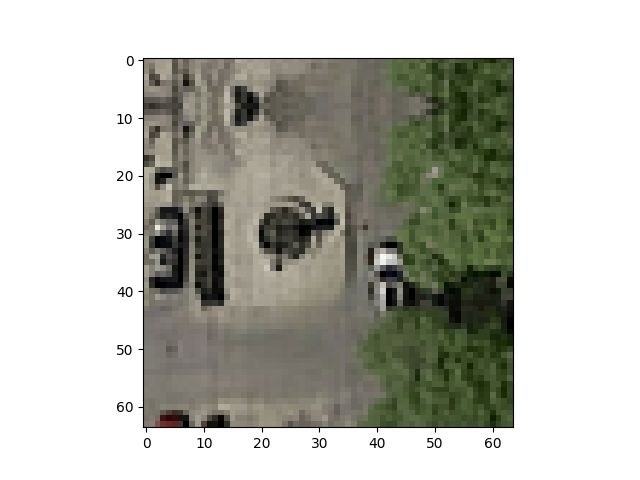
\includegraphics[width=\linewidth]{cont_added_patch.png}
  \caption{Context added patch}
\end{subfigure}
\caption{Different approaches}
\label{fig:patches}
\end{figure}

We have decide for this patch size empirically by trying out different context-added sizes and 64 turned out to bring the
best score on the Kaggle competition\footnote{\url{inclass.kaggle.com/c/cil-road-segmentation-2017}}.

\subsection{Class balancing}
\label{sec:balance}
As our data was very unbalanced i.e. the number of background patches was ~$\times3$ bigger than the number of road patches, 
we had to balance out our data set so that both classes have similar number of representatives. We have done that by 
equalizing the number of patches in both classes, i.e. by randomly picking a limited number of background patches.



\section{Models and Methodsg}
\label{sec:model_and_methods}

\subsection{CNN Architecture}
The core of our work is the CNN design. We have got the main idea for the architecture
of the network from (TODO: cite the paper from which we take the CNN arch.).
Due to limited data and limited computing resources we had to reduce the network substantially. The
reduced version can be described as follows: \\
$IN(3, 64\times64)
-C(64, 3\times3 /2)-C(128, 3\times3 /2)
-C(256, 3\times3 /2)-C(512, 3\times3 /2)
-FC(2048)-FC(2048)-FC(2)$.\\
IN stands for input, C for convolution and FC for fully-connected layers. First number in brackets represents
depth of the layer and the rest represents either the input size or the convolution filter size and the pooling size.
The output of the CNN was the softmax function for the two classes and the optimizer was Adam optimizer \cite{adam}.


\subsection{Error function}
Our CNN model was reducing the log-loss, but for the evaluation we have used two other loss metrics. The first one was
the classification error and it was used on the validation set that helped us find the right number of training epochs. 
Further discussion on that will follow in the next section. The second one was the F-1 score to calculate
the test error. It was given by the Kaggle competition.


\subsection{Model hyper-parameters}
Since we used the Adam optimizer, there were not many parameters to tune. One parameter was the batch size, which we 
have not changed from the baseline model since in the one of previous exercises we have learned the it should nether be too
big nor too small, so we found 32 to be a good choice. The only other parameter to tune was the number of training epochs.
This one we have empirically chosen to be (TODO: state the number) based on training the model on 90 images and 
validating it in every epoch on the other 10 images. The Figure (TODO: ref the plot of validation error) shows
how the validation error changes with the number of epochs. Beside these, there were no further hyper-parameters to tune.


\subsection{Post-processing}
TODO


\section{Results}
\label{sec:results}

TODO
Organize the results section based on the sequence of table and
figures you include. Prepare the tables and figures as soon as all
the data are analyzed and arrange them in the sequence that best
presents your findings in a logical way. A good strategy is to note,
on a draft of each table or figure, the one or two key results you
want to address in the text portion of the results.
The information from the figures is
summarized in Table~\ref{tab:fourier-wavelet}.

\begin{table*}[htbp]
  \centering
  \begin{tabular}[c]{|l||l|l|l|}
    \hline
    Basis&Support&Suitable signals&Unsuitable signals\\
    \hline
    Fourier&global&sine like&localized\\
    wavelet&local&localized&sine like\\
    \hline
  \end{tabular}
  \caption{Characteristics of Fourier and wavelet basis.}
  \label{tab:fourier-wavelet}
\end{table*}

When reporting computational or measurement results, always
report the mean (average value) along with a measure of variability
(standard deviation(s) or standard error of the mean).







\section{Summary}

TODO
The aim of a scientific paper is to convey the idea or discovery of
the researcher to the minds of the readers. The associated software
package provides the relevant details, which are often only briefly
explained in the paper, such that the research can be reproduced.
To write good papers, identify your key idea, make your contributions
explicit, and use examples and illustrations to describe the problems
and solutions.



\bibliographystyle{IEEEtran}
\bibliography{howto-paper}
\end{document}
